%%
%  ******************************************************************************
%  * #file    Szablon_raportu_EN_Latex.tex
%  * #author  Adrian Wójcik   adrian.wojcik(at)put.poznan.pl
%  *          
%  * #commit  Patryk Kościk   koscikpatryk(at)gmail.com
%  *          Modified the template for Projekt przejsciowy purposes          
%  *          
%  *
%  * #commit  Patryk Kościk   koscikpatryk(at)gmail.com
%  *          Zupełnie przewrócono na łeb formatke po taktycznym wyjasnieniu          
%  *          
%  * #version 1.1
%  * #date    09-Mar-2022
%  * #brief   PROJPRZEJ
%  *
%  ******************************************************************************
%%  
\documentclass[11pt, a4paper]{article}

\usepackage{SM_template}

% Wypełnijcie te dyrektywy zgodnie z waszym tematem
%
% \lab      -> NAZWA CZUJNIKA,          np.: 'DHT22'
% \comment  -> Króciutki opis co to,    np.: 'Cyfrowy czujnik temperatury'
% \author   -> Autor dokumentu          np.: Patryk Kościk
%
% Pamiętajcie o zmianie ścieżki w \addbibresourcue (!)

\lab{Czujnik dotyku KY-036}
\comment{Czujnik analogowy z dotatkowym binarynym wyjściem progującym}
\author{Patryk Kościk}
\addbibresource{bib/KY-017.bib}

%
% Początek dokumentu
%
\begin{document}

%
% Strona tytułowa
%
\mainpage{KY-036/KY-036.jpg}
\newpage

\section*{Opis elementu}
Sercem czujnika jest tranzystor modelu KSP13, który jest tranzystorem w układzie Darlingtona (\ref{fig:_zdjecie_elementu}). Ten rodzaj połączenia charakteryzuje bardzo duży współczynnik wzmocnienia stałoprądowego ($\beta$ lub $h_{FE}$). Tranzystory w standardowych konfiguracjach cechują się wzmocnieniem rzędu od 100 do 300. Omawiany KSP13 gwarantuje wzmocnienie równe conajmniej 10000.

Dodatkowo w module KY-036, baza tranzystora jest tzw. \textit{floating}, czyli niepodłączona do czegokolwiek. Taka konfiguracja połączona z dużym współczynnikiem wzmocnienia, cechuje się tym że, wystarczy najmniejsza perturbacja na bazie, aby wprowadzić tranzystor w stan przewodzenia.

%%%%%%%%%%%%%%%%%%%%%%%%%  TWO IMAGES SIDE BY SIDE  %%%%%%%%%%%%%%%%%%%%%%%%%%%%%
\vspace{0.25cm}
\begin{figure}[h]
\centering
%%%%%%%%%%%%%%%%%%%%%%%%%%%%%%%%%%%%%%%%%%%%%%%%%%%%%%%%%%%%%%%%%%%%%%%%%%%%%%%%%
\begin{subfigure}{.5\textwidth}
\centering
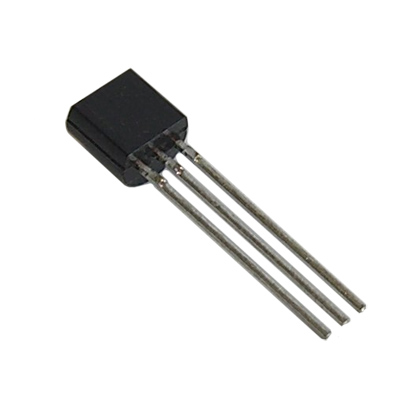
\includegraphics[width=.7\linewidth]{fig/KY-036/hi-1064-065920-TO-92.jpg}
\caption{Zdjęcie Tranzystora KSP13}
\label{fig:_zdjecie_elementu}
\end{subfigure}%
%%%%%%%%%%%%%%%%%%%%%%%%%%%%%%%%%%%%%%%%%%%%%%%%%%%%%%%%%%%%%%%%%%%%%%%%%%%%%%%%%
\begin{subfigure}{.5\textwidth}
\centering
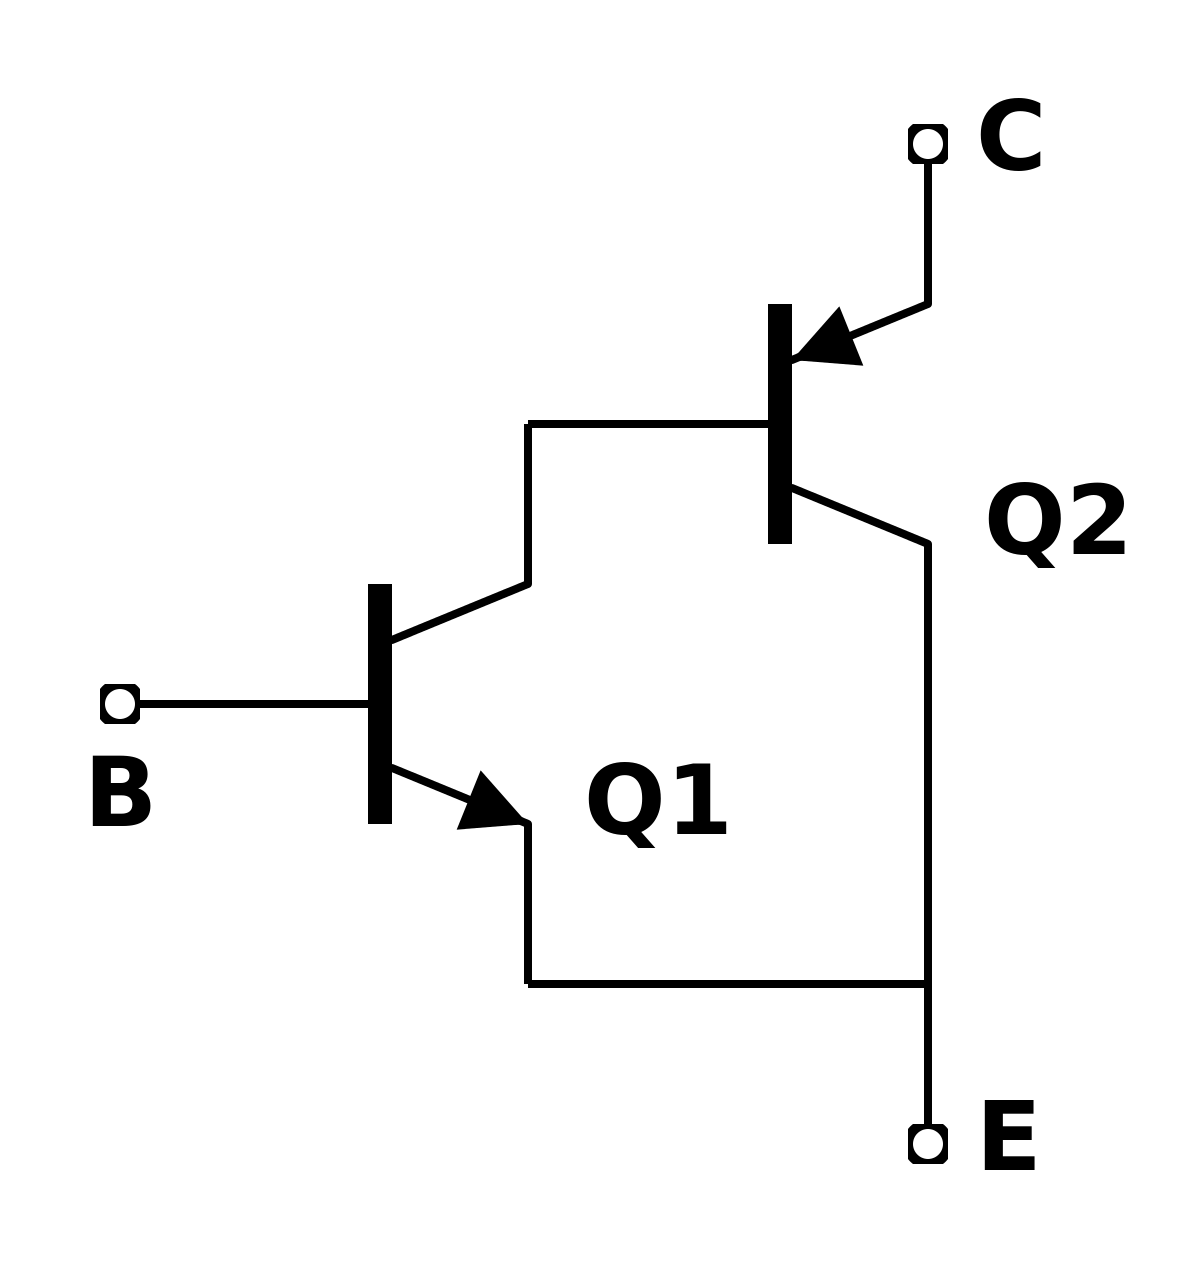
\includegraphics[width=.7\linewidth]{fig/KY-036/1200px-Compound_trans.svg.png}
\caption{Zasada działania pary Darlingtona: $h_{FE} = h_{q1} \cdot h_{q2}$}
\label{fig:_zasada_dzialania_elementu}
\end{subfigure}
%%%%%%%%%%%%%%%%%%%%%%%%%%%%%%%%%%%%%%%%%%%%%%%%%%%%%%%%%%%%%%%%%%%%%%%%%%%%%%%%%
% \caption{PODPIS}
\label{fig:element}
\end{figure}
\vspace{0.25cm}
%%%%%%%%%%%%%%%%%%%%%%%%%  TWO IMAGES SIDE BY SIDE  %%%%%%%%%%%%%%%%%%%%%%%%%%%%%



% \subsection{Opis modułu} REPLACE SUBSECTION WITH 1CM VSPACE
\vspace{0.75cm}

Moduł sensora wykrycia dotyku, wykorzystuje wyżej opisane właściwości elementu, umożliwiając bezpieczne i tanie wykrywanie dotyku. Moduł ten, poza elementami pasywnymi, składa się z zestawu wzmacniaczy operacyjnych \textbf{LM393}, służących jako układ progowania, trymera do regulacji czułości (\textit{threshold}) układu progowania, oraz dwóch elementów LED sygnalizujących zasilanie oraz pobudzenie czujnika. 

%%%%%%%%%%%%%%%%%%%%%%%%%  TWO IMAGES SIDE BY SIDE  %%%%%%%%%%%%%%%%%%%%%%%%%%%%%
\begin{figure}[h]
\centering
%%%%%%%%%%%%%%%%%%%%%%%%%%%%%%%%%%%%%%%%%%%%%%%%%%%%%%%%%%%%%%%%%%%%%%%%%%%%%%%%%
\begin{subfigure}{.5\textwidth}
\centering
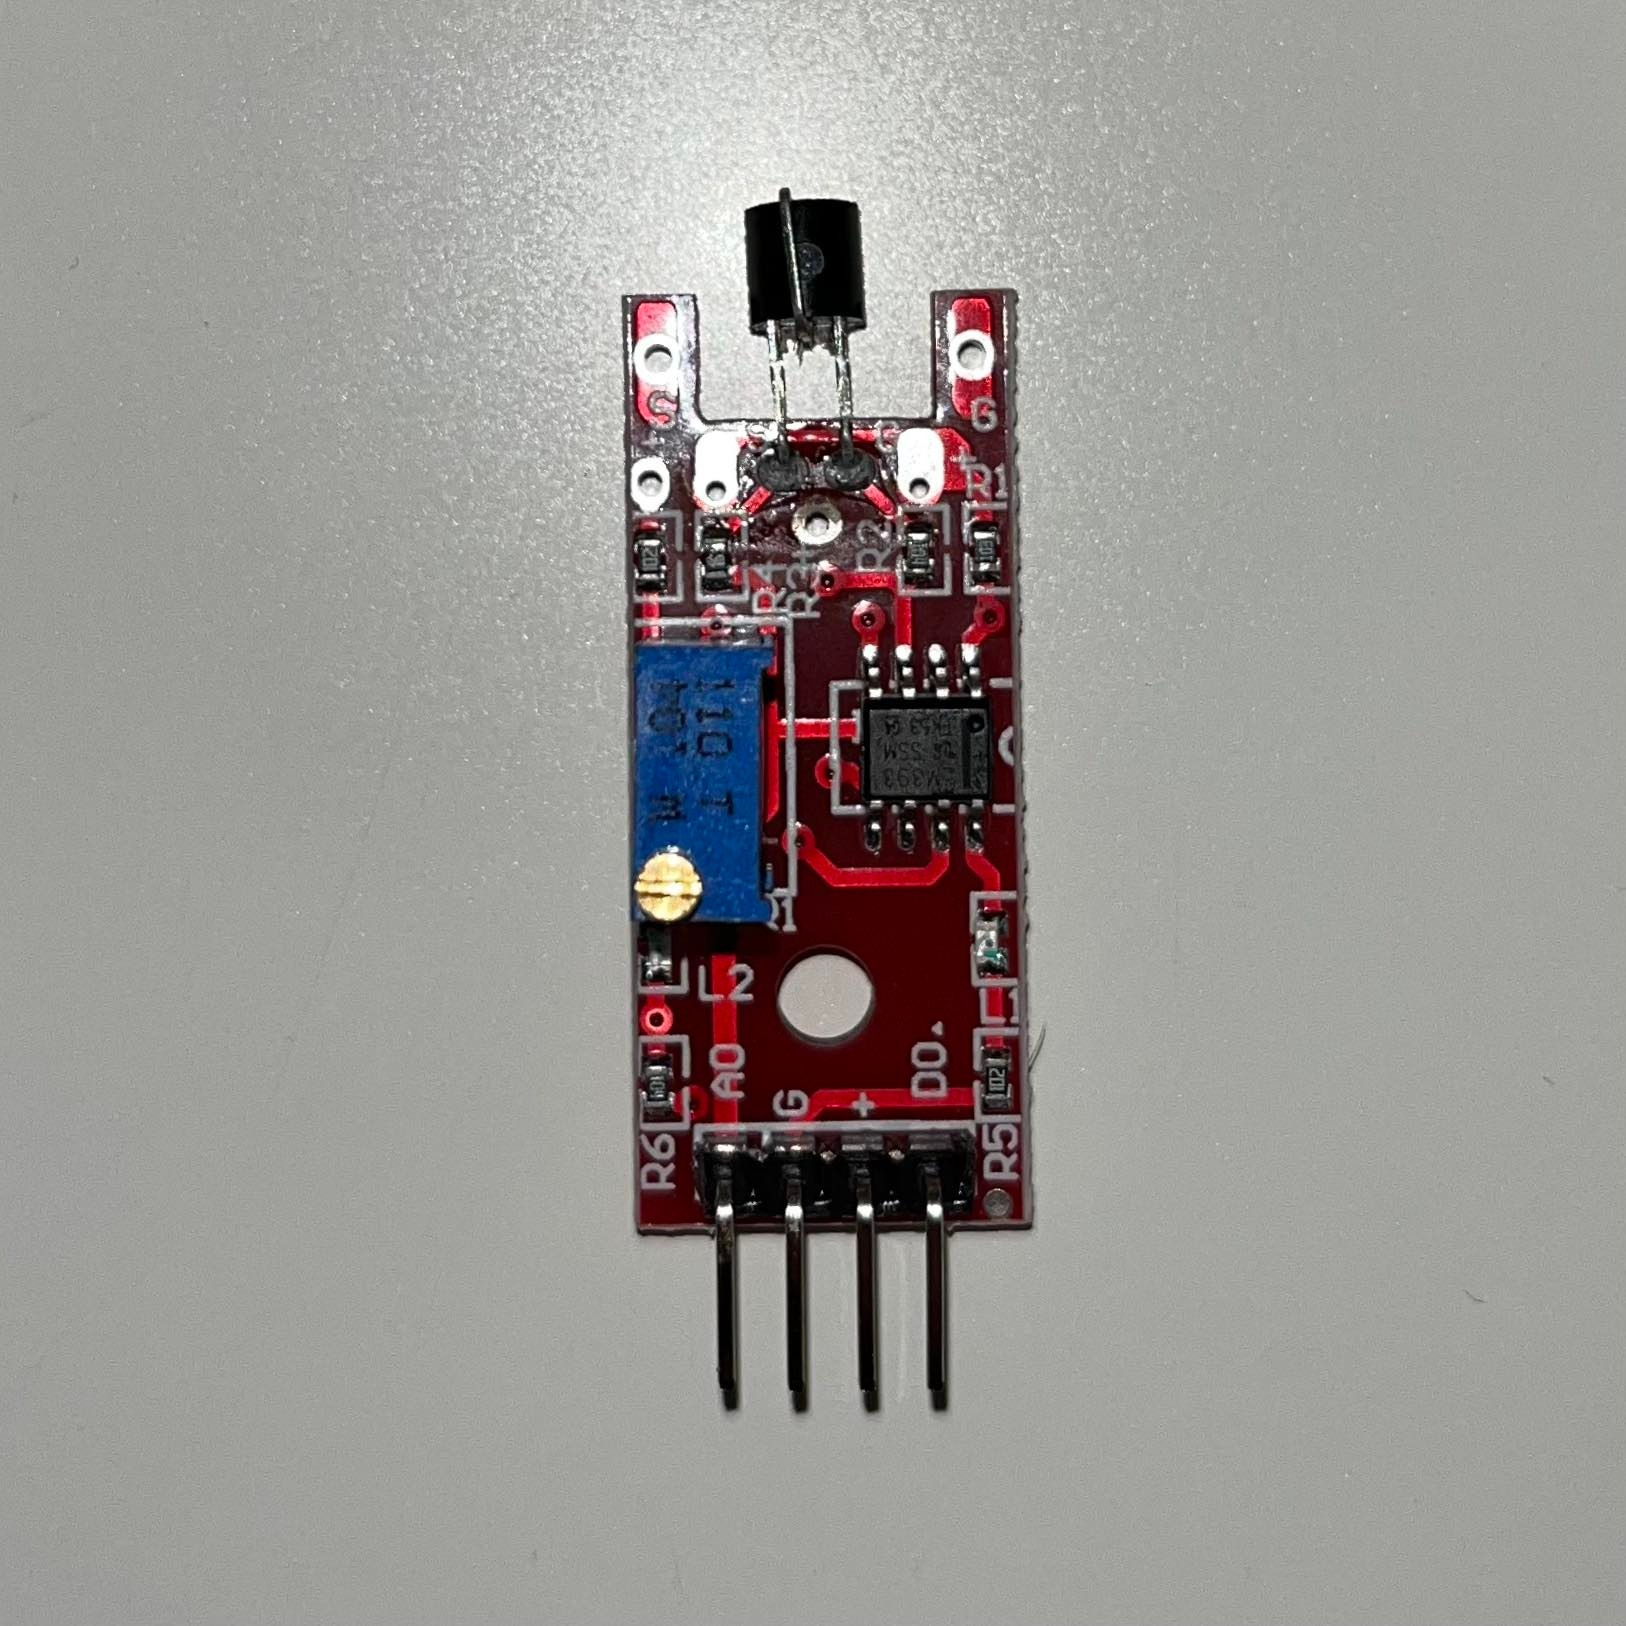
\includegraphics[width=.7\linewidth]{fig/KY-036/283965536_377900227645925_1471273661785834276_n.jpg}
\caption{Zdjęcie modułu}
\label{fig:_zdjecie_modulu}
\end{subfigure}%
%%%%%%%%%%%%%%%%%%%%%%%%%%%%%%%%%%%%%%%%%%%%%%%%%%%%%%%%%%%%%%%%%%%%%%%%%%%%%%%%%
\begin{subfigure}{.5\textwidth}
\centering
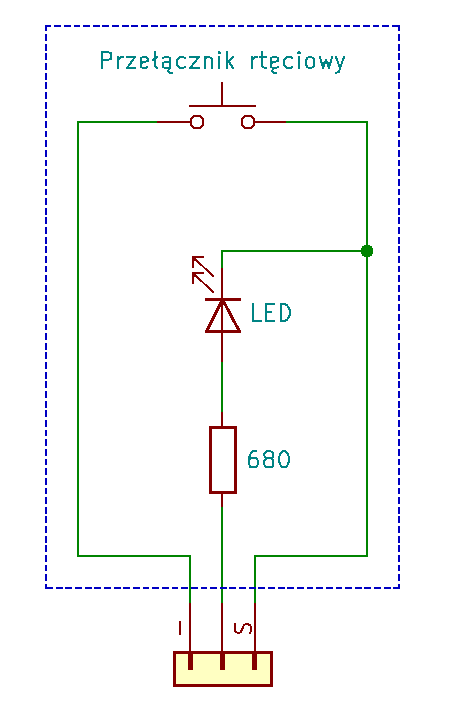
\includegraphics[width=.5\linewidth]{fig/KY-017/zdj_modułu/modul.png}
\caption{Schemat modułu}

\end{subfigure}
%%%%%%%%%%%%%%%%%%%%%%%%%%%%%%%%%%%%%%%%%%%%%%%%%%%%%%%%%%%%%%%%%%%%%%%%%%%%%%%%%
\label{fig:modul}
\end{figure}
\vspace{0.5cm}
%%%%%%%%%%%%%%%%%%%%%%%%%  TWO IMAGES SIDE BY SIDE  %%%%%%%%%%%%%%%%%%%%%%%%%%%%%

\newpage

\begin{figure}[h!]
    \centering
    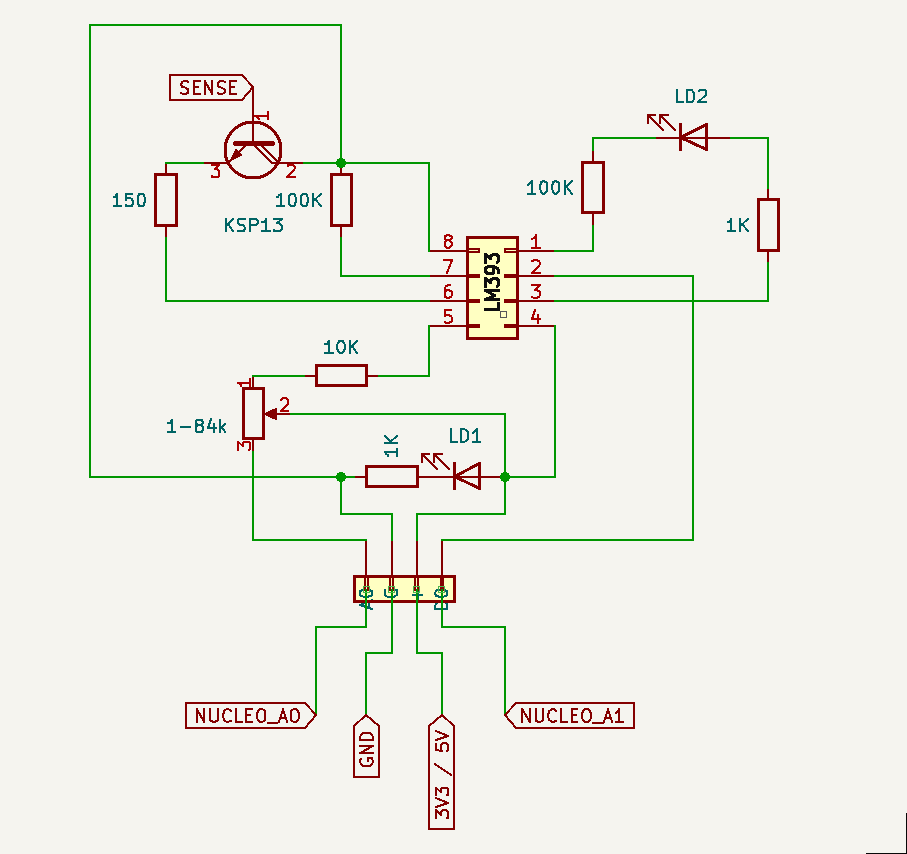
\includegraphics[width=0.7\textwidth]{fig/KY-036/284156354_331751615703128_964279712853339648_n.png}
    \caption{Ogólny schemat elektryczny modułu KY-036.}
    \label{fig:_schemat_modulu}
\end{figure}


\newpage

\section{Użycie czujnika}
\subsection{Bez mikrokontrolera}
\subsubsection{Wyjście progujące}

Działanie czujnika w trybie wyjścia progującego możemy zweryfikować, bez użycia mikrokontrolera, podłączając multimetr
w trybie woltomierza, do pinów \texttt{D0} oraz \texttt{-}.

% TUTAJ FOTY ODNOSNIE TEGO
%%%%%%%%%%%%%%%%%%%%%%%%%  TWO IMAGES SIDE BY SIDE  %%%%%%%%%%%%%%%%%%%%%%%%%%%%%
\vspace{0.25cm}
\begin{figure}[h]
\centering
%%%%%%%%%%%%%%%%%%%%%%%%%%%%%%%%%%%%%%%%%%%%%%%%%%%%%%%%%%%%%%%%%%%%%%%%%%%%%%%%%
\begin{subfigure}{.5\textwidth}
\centering
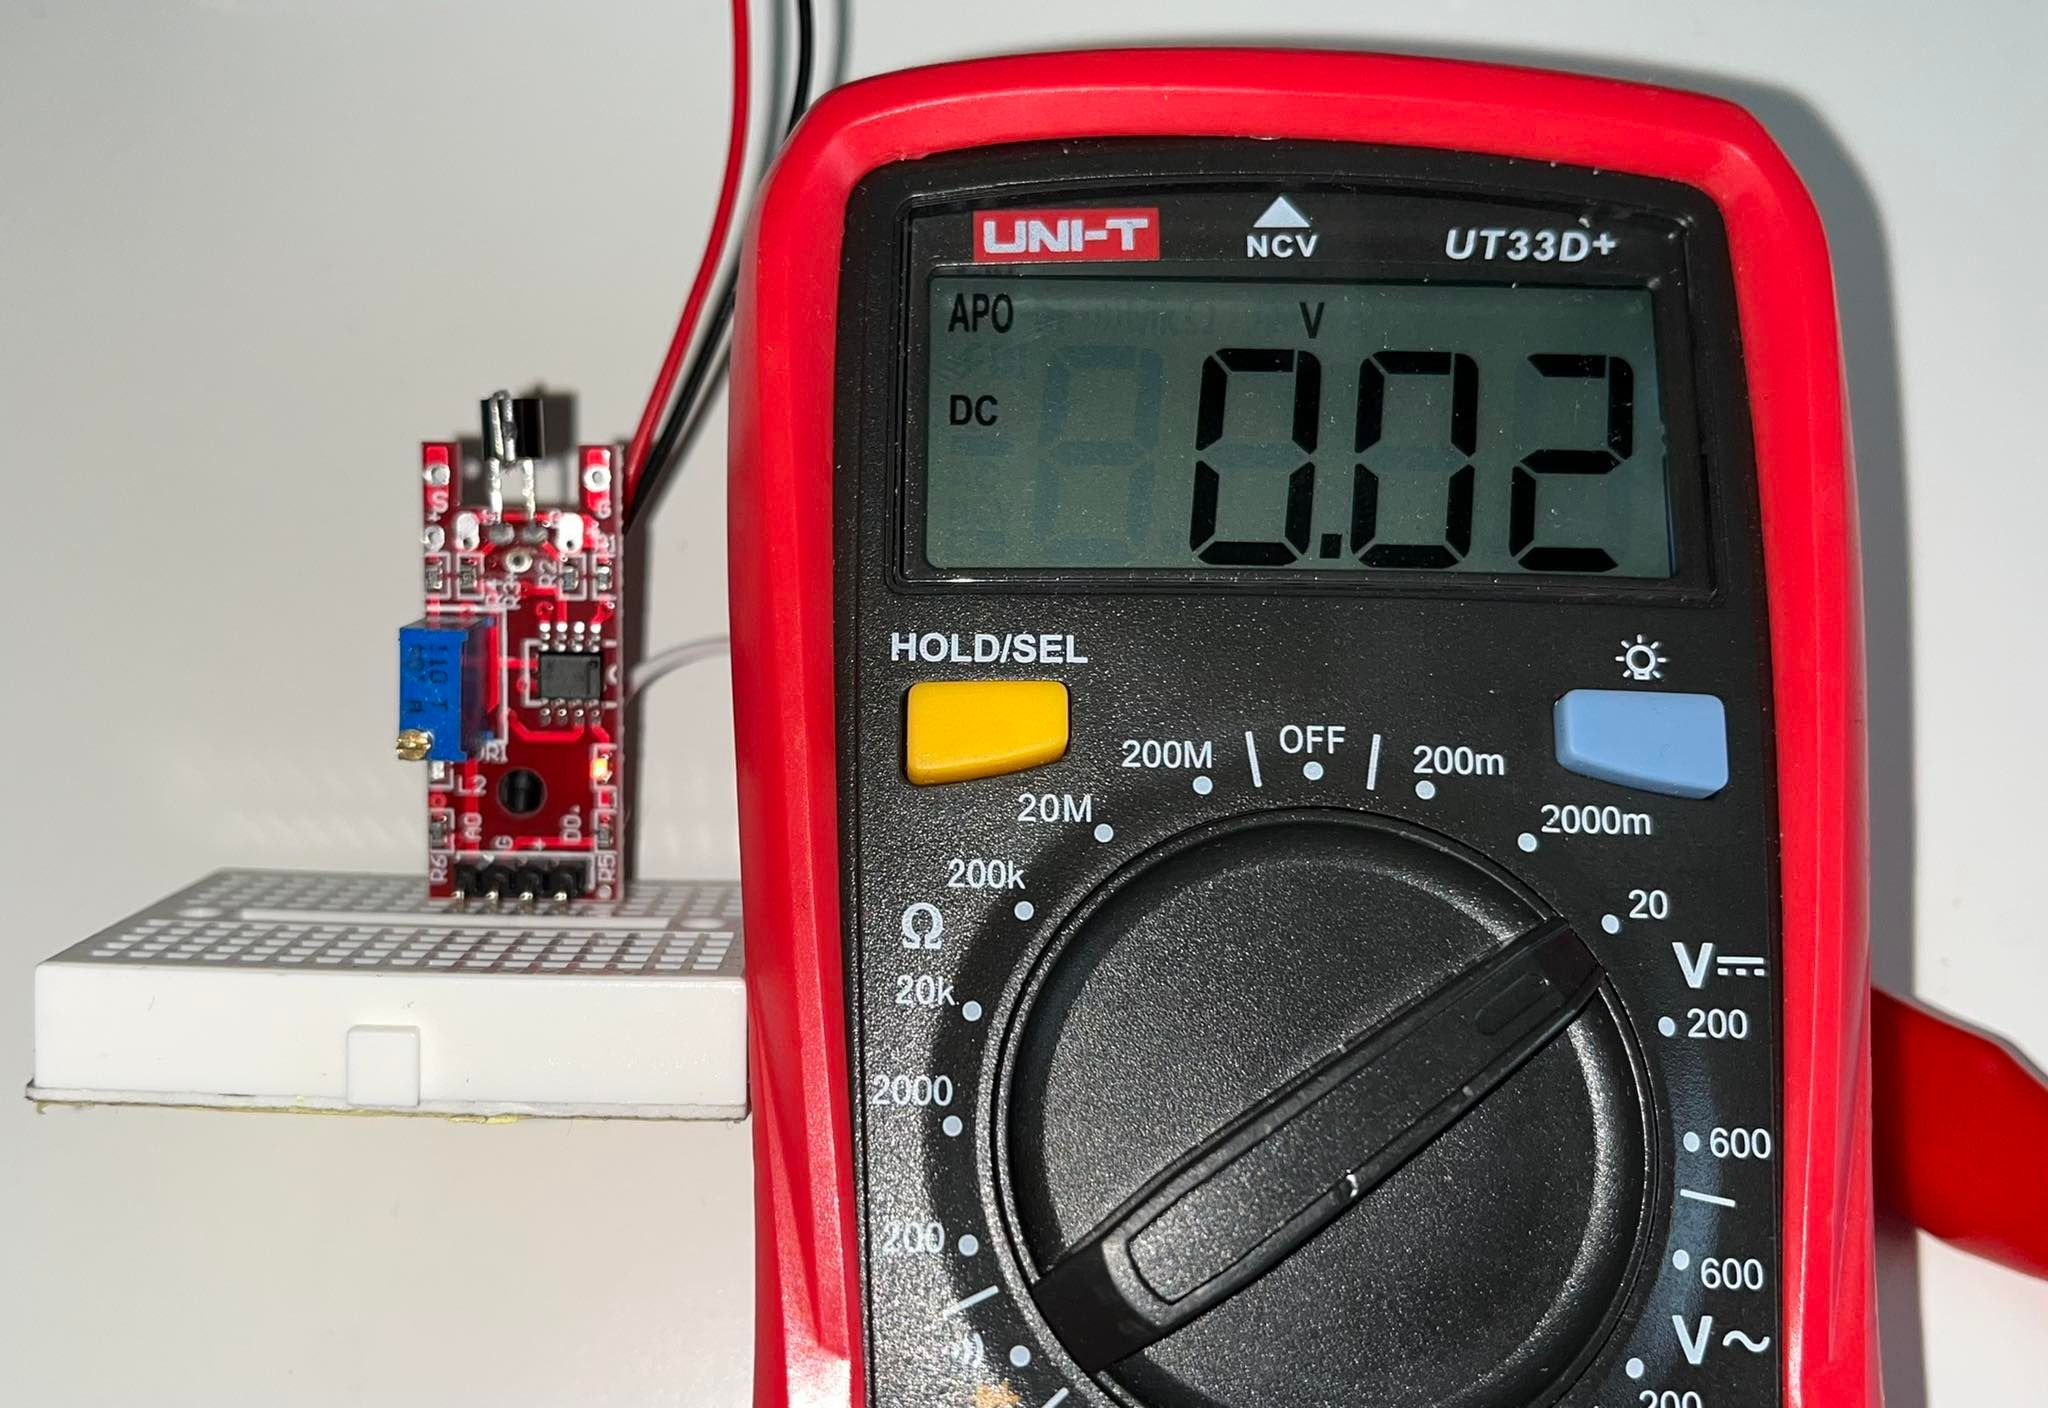
\includegraphics[width=.9\linewidth]{fig/KY-036/283758226_769757180846069_2450086641381727927_n}
\caption{Brak dotyku - stan niski}
\label{fig:_uklad_woltomierz_otw}
\end{subfigure}%
%%%%%%%%%%%%%%%%%%%%%%%%%%%%%%%%%%%%%%%%%%%%%%%%%%%%%%%%%%%%%%%%%%%%%%%%%%%%%%%%%
\begin{subfigure}{.5\textwidth}
\centering
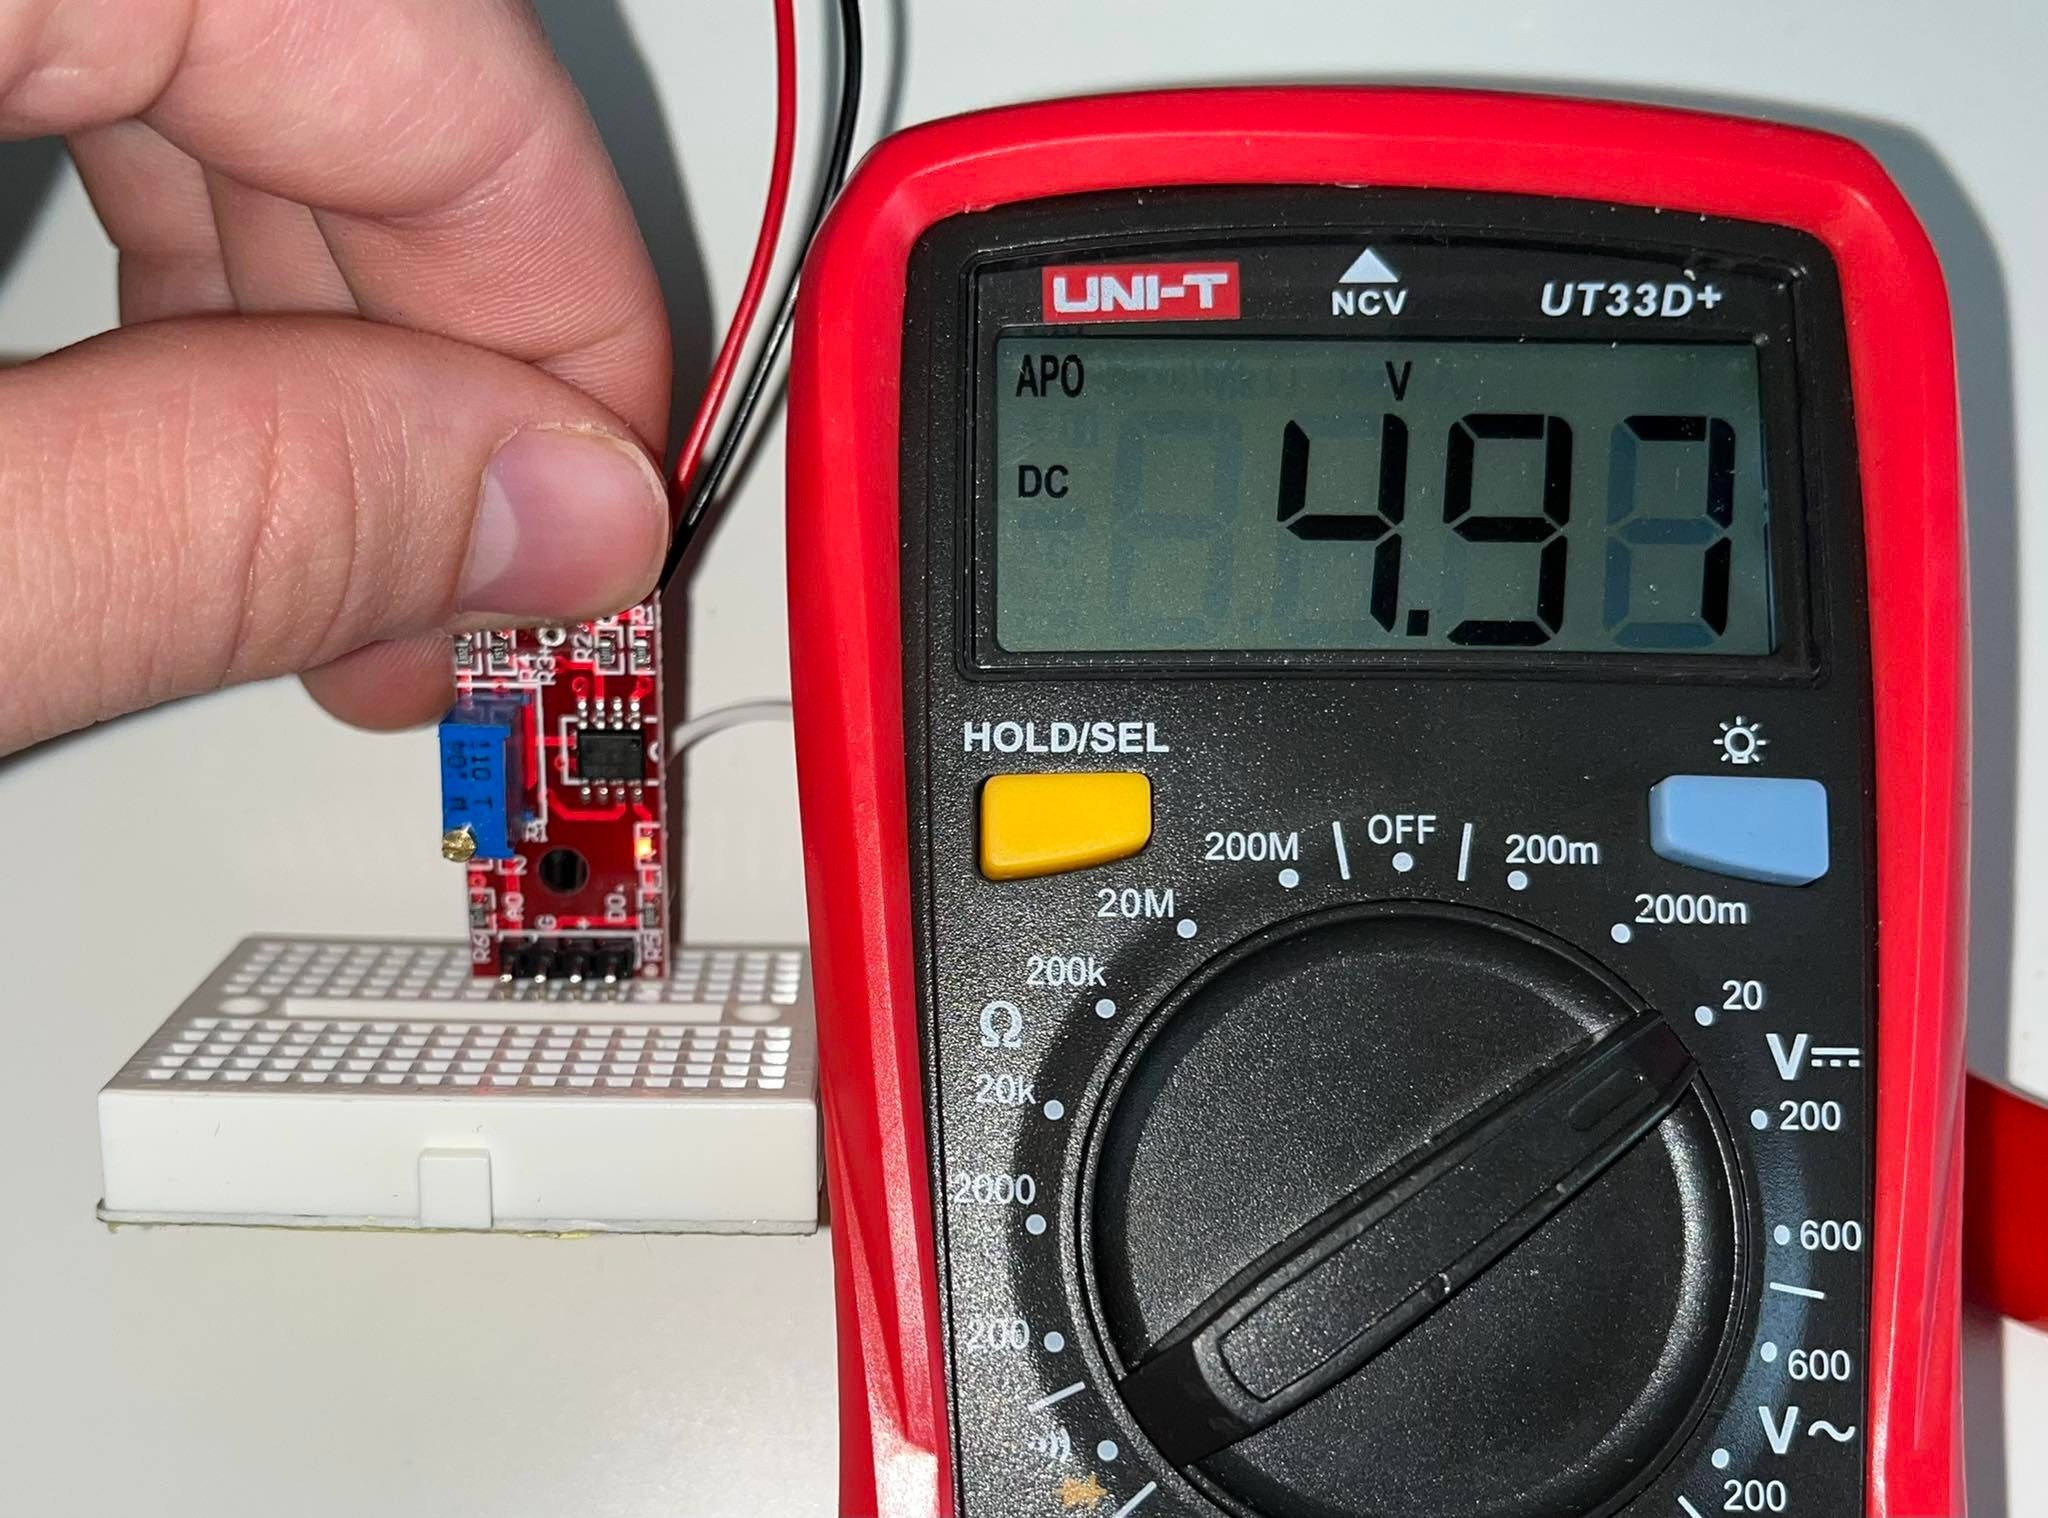
\includegraphics[width=.9\linewidth]{fig/KY-036/281631346_529764192182061_5396655729694026560_n}
\caption{Obecność dotyku - stan wysoki}
\label{fig:_uklad_woltomierz_zmk}
\end{subfigure}
%%%%%%%%%%%%%%%%%%%%%%%%%%%%%%%%%%%%%%%%%%%%%%%%%%%%%%%%%%%%%%%%%%%%%%%%%%%%%%%%%
% \caption{PODPIS}
\label{fig:woltomierz}
\end{figure}
\vspace{0.25cm}
%%%%%%%%%%%%%%%%%%%%%%%%%  TWO IMAGES SIDE BY SIDE  %%%%%%%%%%%%%%%%%%%%%%%%%%%%%

\subsubsection{Wyjście analogowe}
Działanie czujnika w trybie wyjścia analogowego możemy zweryfikować, bez użycia mikrokontrolera, podłączając multimetr
w trybie woltomierza, do pinów \texttt{A0} oraz \texttt{-}.

% TUTAJ FOTY ODNOSNIE TEGO
%%%%%%%%%%%%%%%%%%%%%%%%%  TWO IMAGES SIDE BY SIDE  %%%%%%%%%%%%%%%%%%%%%%%%%%%%%
\vspace{0.25cm}
\begin{figure}[h]
\centering
%%%%%%%%%%%%%%%%%%%%%%%%%%%%%%%%%%%%%%%%%%%%%%%%%%%%%%%%%%%%%%%%%%%%%%%%%%%%%%%%%
\begin{subfigure}{.5\textwidth}
\centering
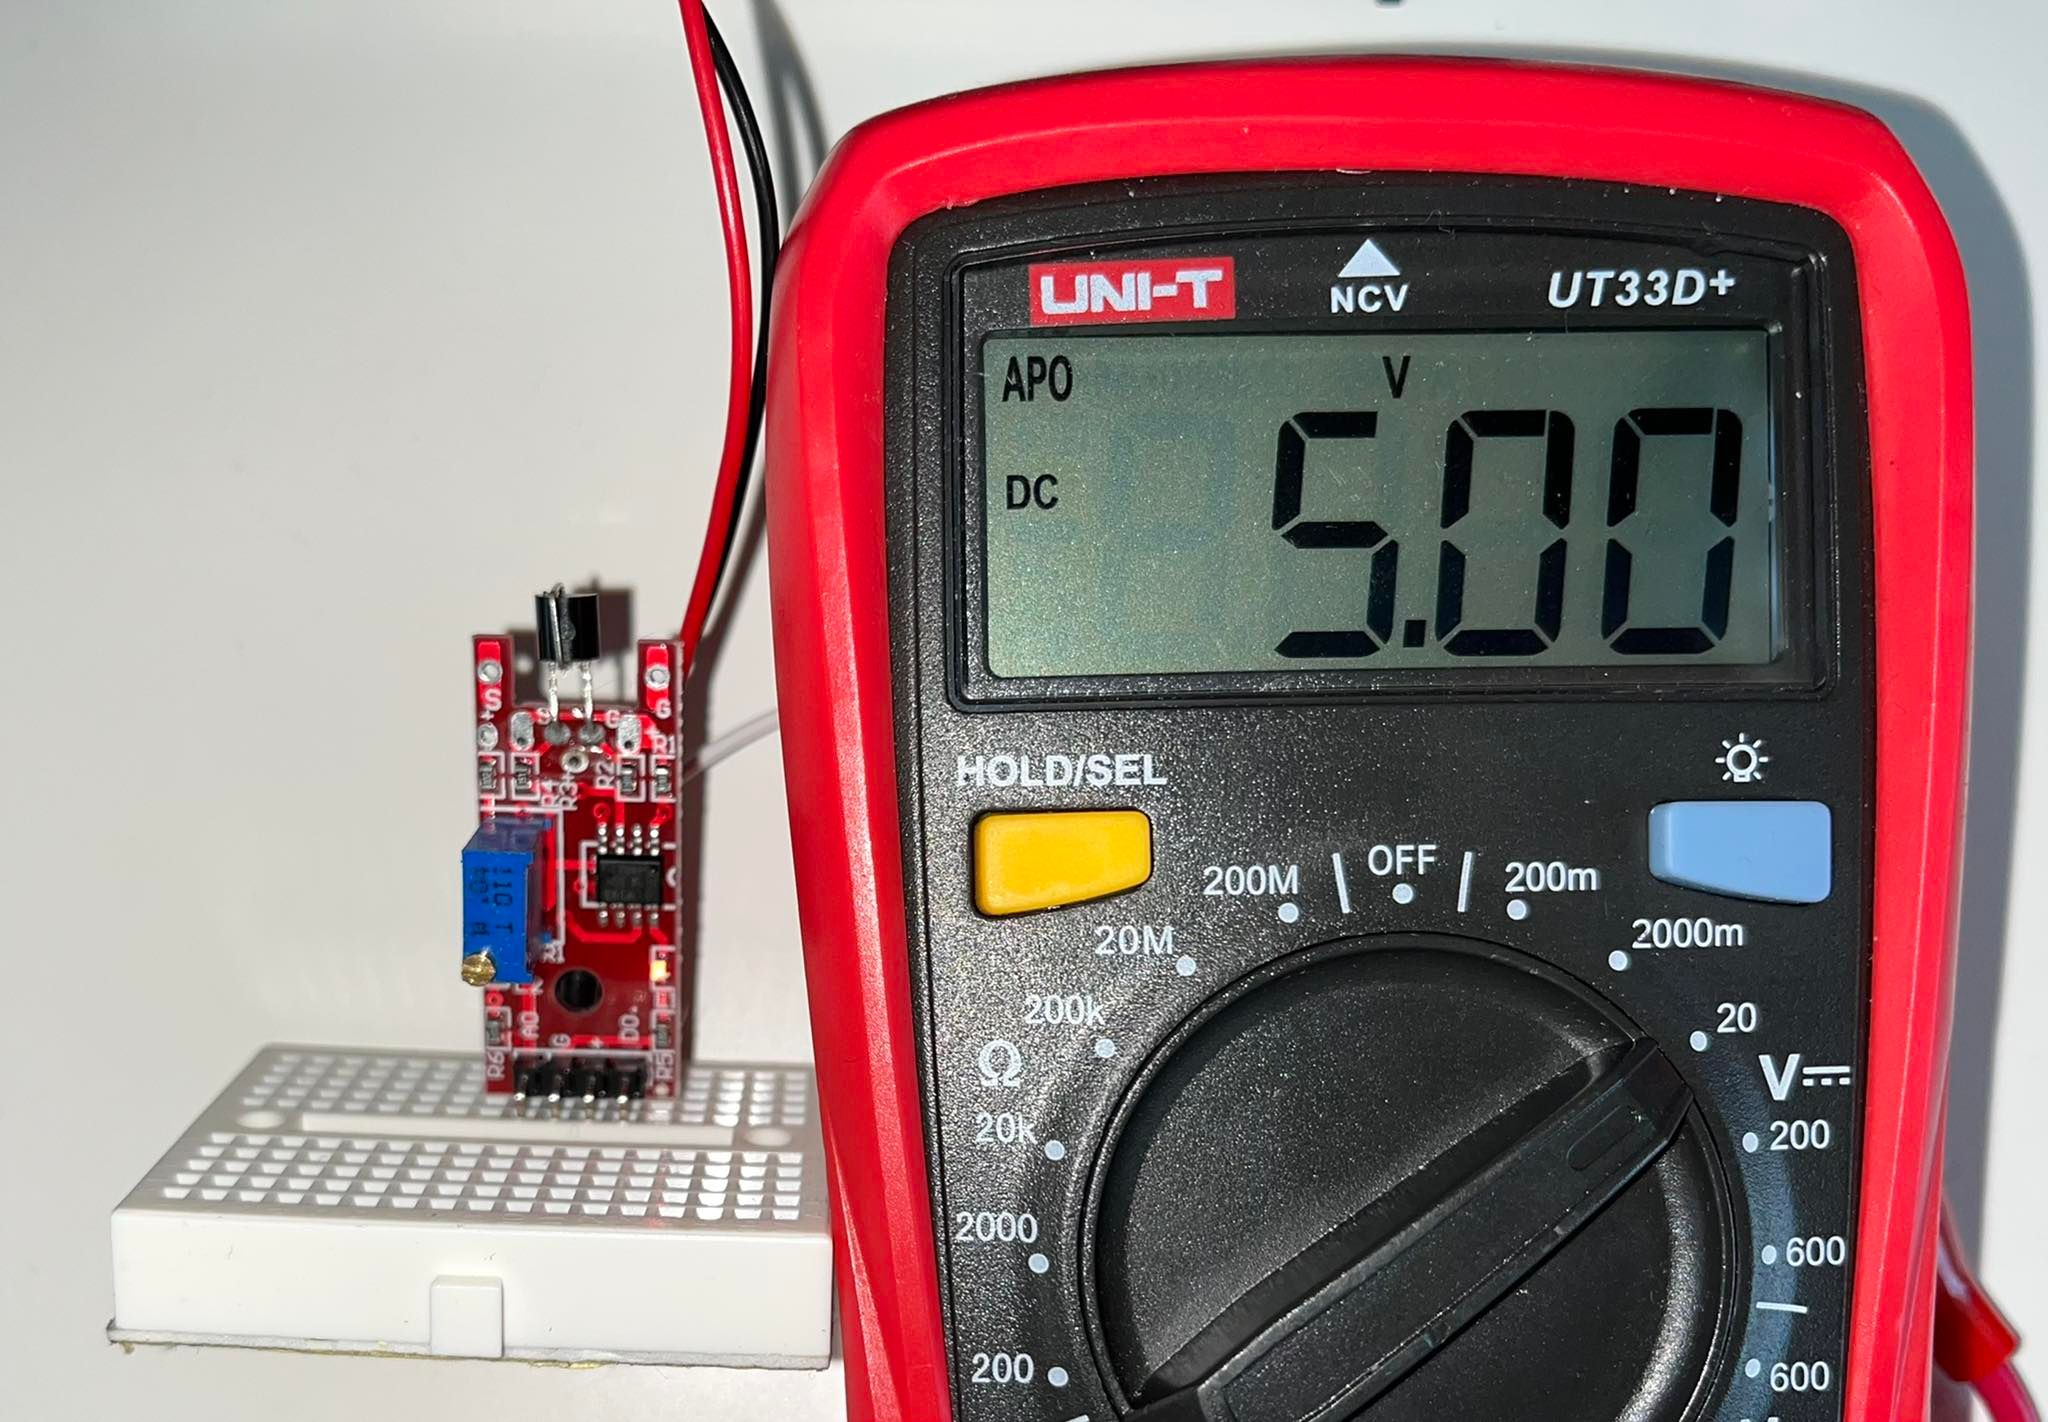
\includegraphics[width=.9\linewidth]{fig/KY-036/282820859_337533828451797_8222466624857442728_n}
\caption{Brak dotyku - Napięcie \textit{A0} = 5V}
\label{fig:_uklad_woltomierz_otw}
\end{subfigure}%
%%%%%%%%%%%%%%%%%%%%%%%%%%%%%%%%%%%%%%%%%%%%%%%%%%%%%%%%%%%%%%%%%%%%%%%%%%%%%%%%%
\begin{subfigure}{.5\textwidth}
\centering
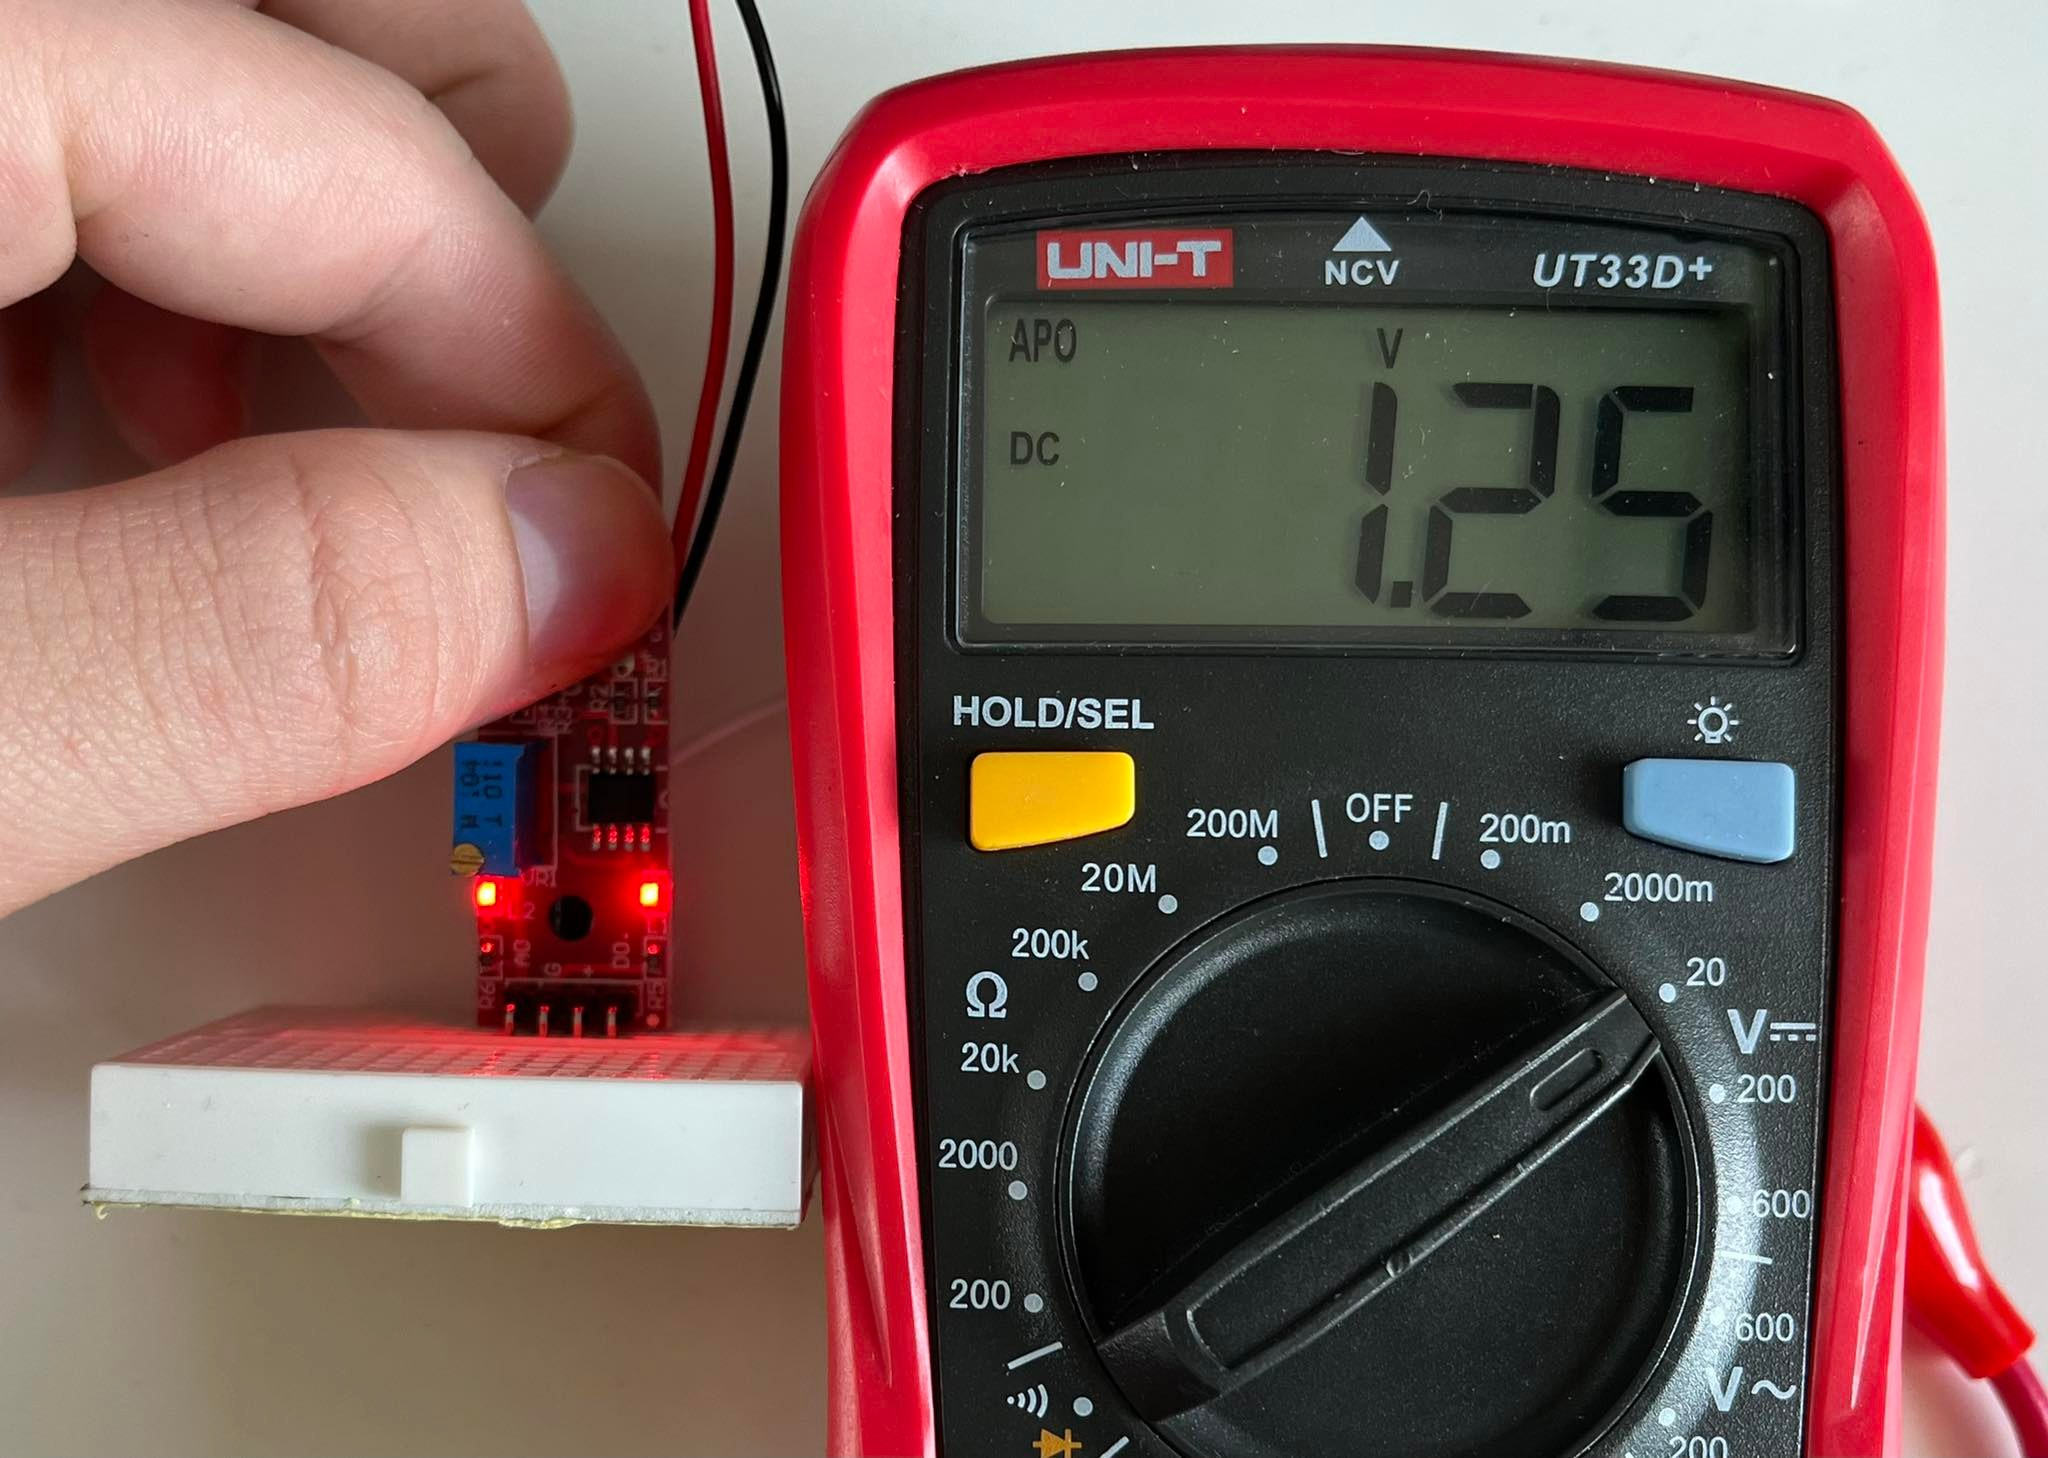
\includegraphics[width=.9\linewidth]{fig/KY-036/282838602_740656317115777_5297824243567198867_n}
\caption{Obecność dotyku - Napięcie \textit{A0} $\approx$ 1.25V}
\label{fig:_uklad_woltomierz_zmk}
\end{subfigure}
%%%%%%%%%%%%%%%%%%%%%%%%%%%%%%%%%%%%%%%%%%%%%%%%%%%%%%%%%%%%%%%%%%%%%%%%%%%%%%%%%
% \caption{PODPIS}
\label{fig:woltomierz}
\end{figure}
\vspace{0.25cm}

Czujnik działa następująco
\begin{itemize}
    \item W połączeniu binarnym: brak dotyku - stan niski, obecność dotyku - stan wysoki = $V_{cc}$
    \item W połączeniu analogowym: brak dotyku - $A0 = V_{cc}$, obecność dotyku - $A0 \approx 1.25 V$
\end{itemize}

Dodatkowo można zaobserwować diodę po lewej stronie, sygnalizującą stan wyjścia binarnego czujnika.

\newpage
\subsection{Mikrokontroler}
\subsubsection{Wyjście binarne}
Oczywiście czujnik możemy używac w połączeniu z mikrokontrolerem. Schemat połączeń i konfiguracja
mikrokontrolera została opisana w sekcji \texttt{Suplement \#1}.Zawiera tam się również kod języka
C + HAL, pozwalający odczytać wartości z czujnika.

Kod jest skonfigurowany tak, aby uruchamiał wbudowany w płytkę mikrokontrolera element LED. Na 
zdjęciach dodatkowo widać działanie wbudowanej w moduł diody LED. 

% TUTAJ FOTY ODNOSNIE TEGO
%%%%%%%%%%%%%%%%%%%%%%%%%  TWO IMAGES SIDE BY SIDE  %%%%%%%%%%%%%%%%%%%%%%%%%%%%%
\vspace{0.25cm}
\begin{figure}[h]
\centering
%%%%%%%%%%%%%%%%%%%%%%%%%%%%%%%%%%%%%%%%%%%%%%%%%%%%%%%%%%%%%%%%%%%%%%%%%%%%%%%%%
\begin{subfigure}{.5\textwidth}
\centering
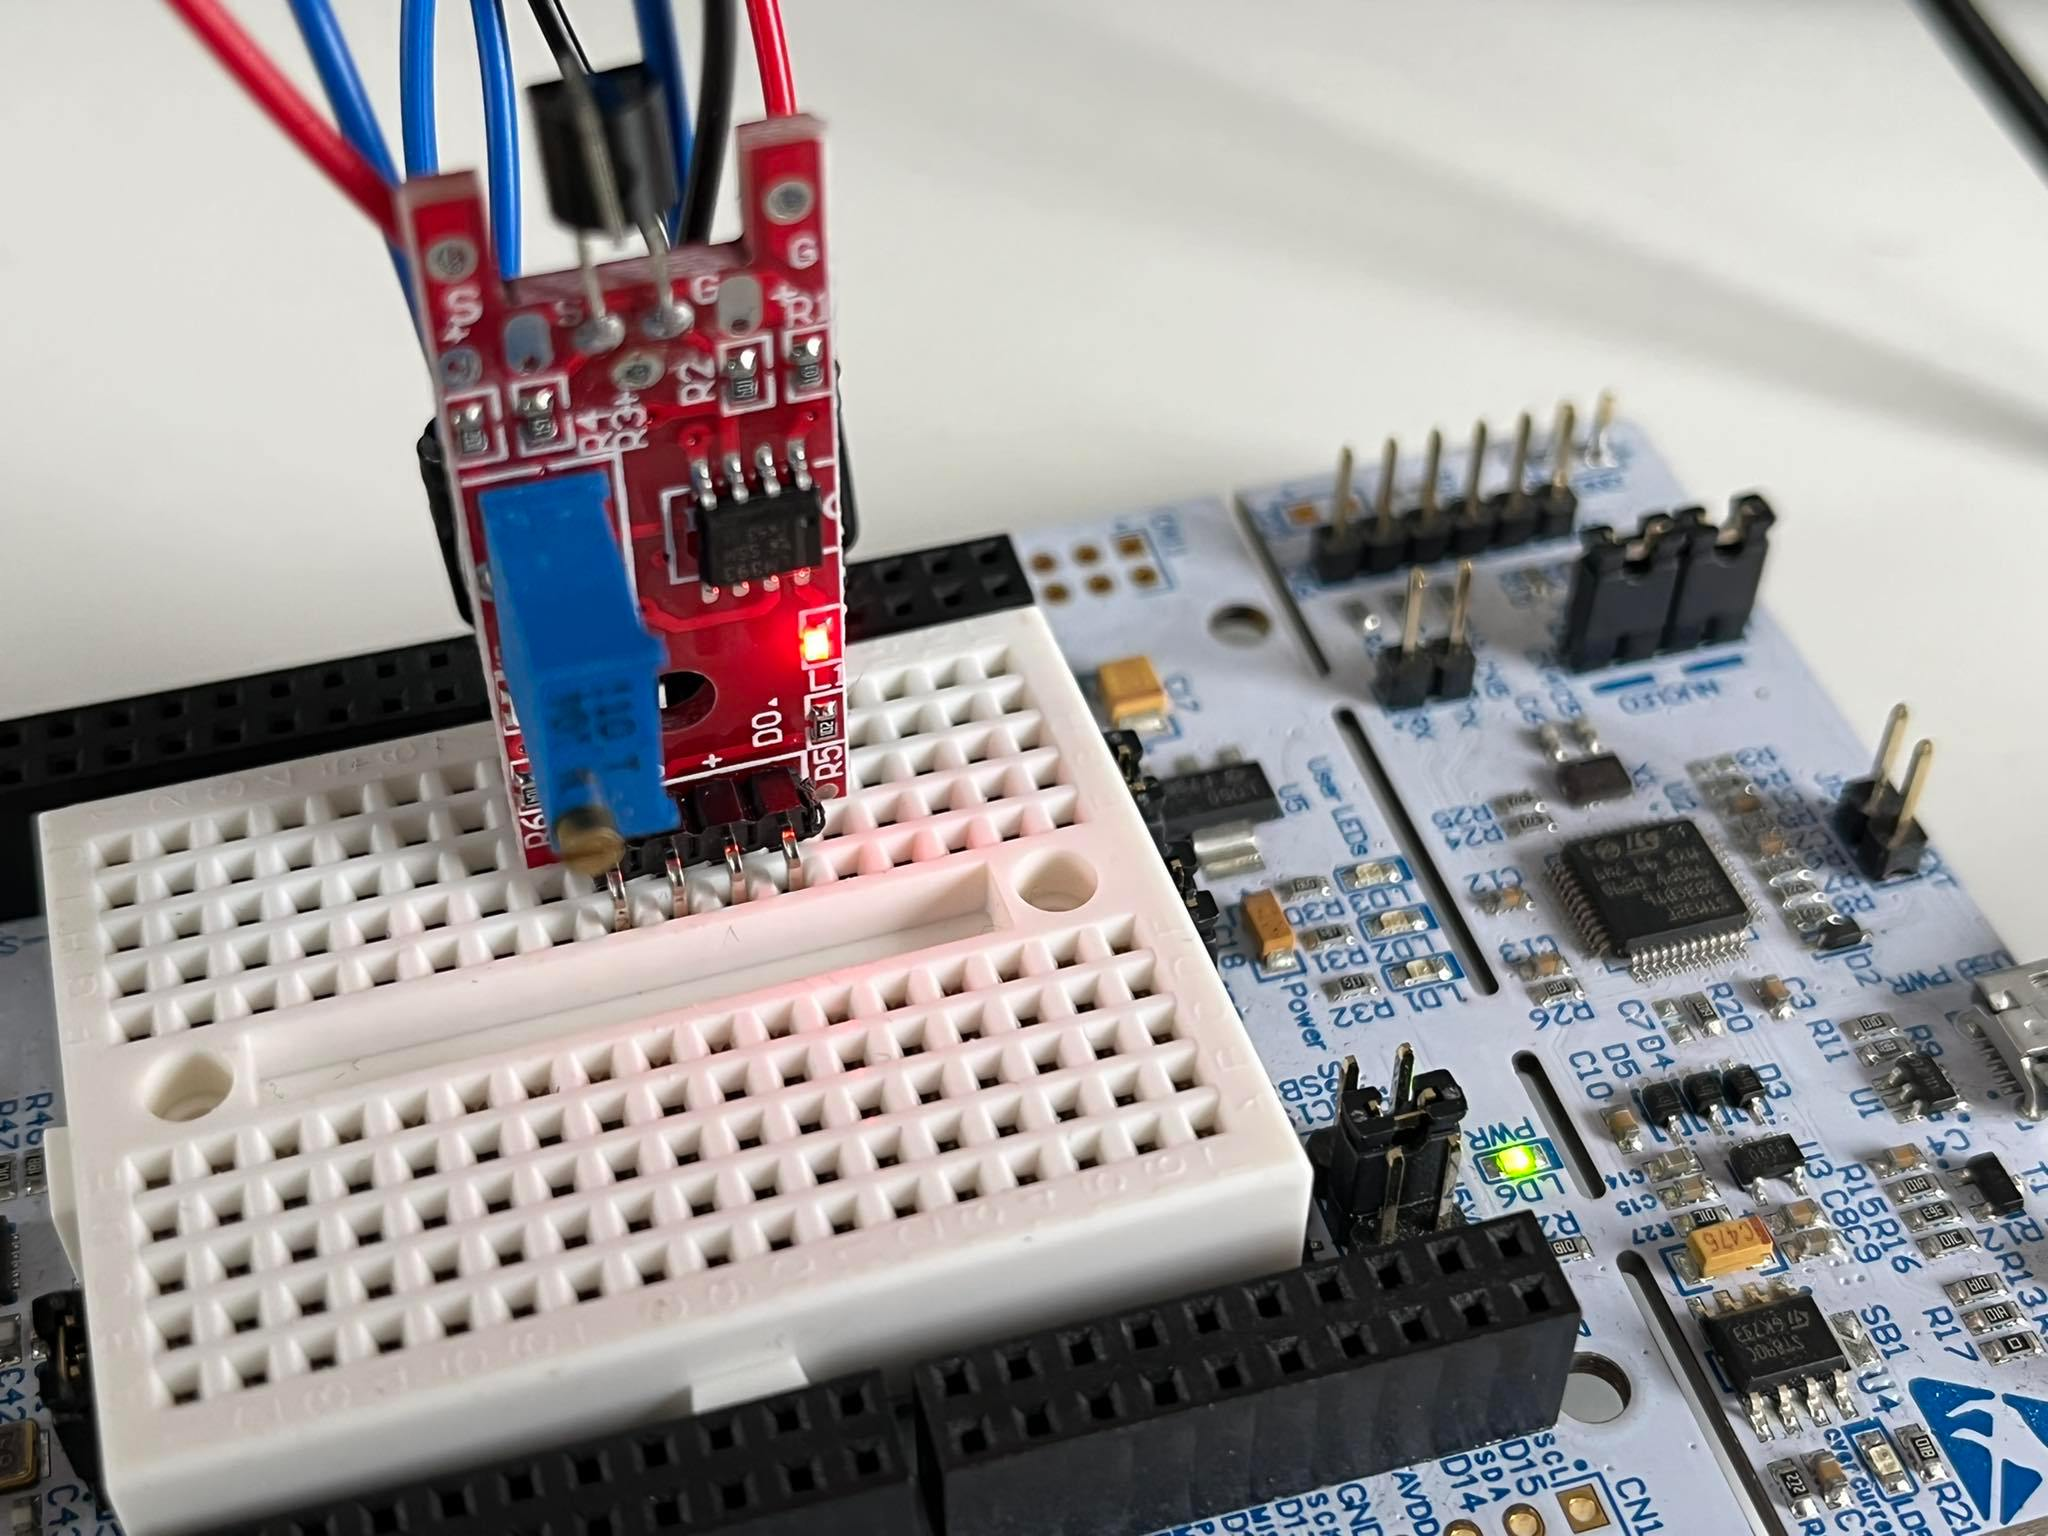
\includegraphics[width=.9\linewidth]{fig/KY-036/284806248_540548144336070_8978676119647820502_n}
\caption{Dioda LD1 wyłączona podczas braku dotyku}
\label{fig:_układ_mikroproc_dioda_wyl}
\end{subfigure}%
%%%%%%%%%%%%%%%%%%%%%%%%%%%%%%%%%%%%%%%%%%%%%%%%%%%%%%%%%%%%%%%%%%%%%%%%%%%%%%%%%
\begin{subfigure}{.5\textwidth}
\centering
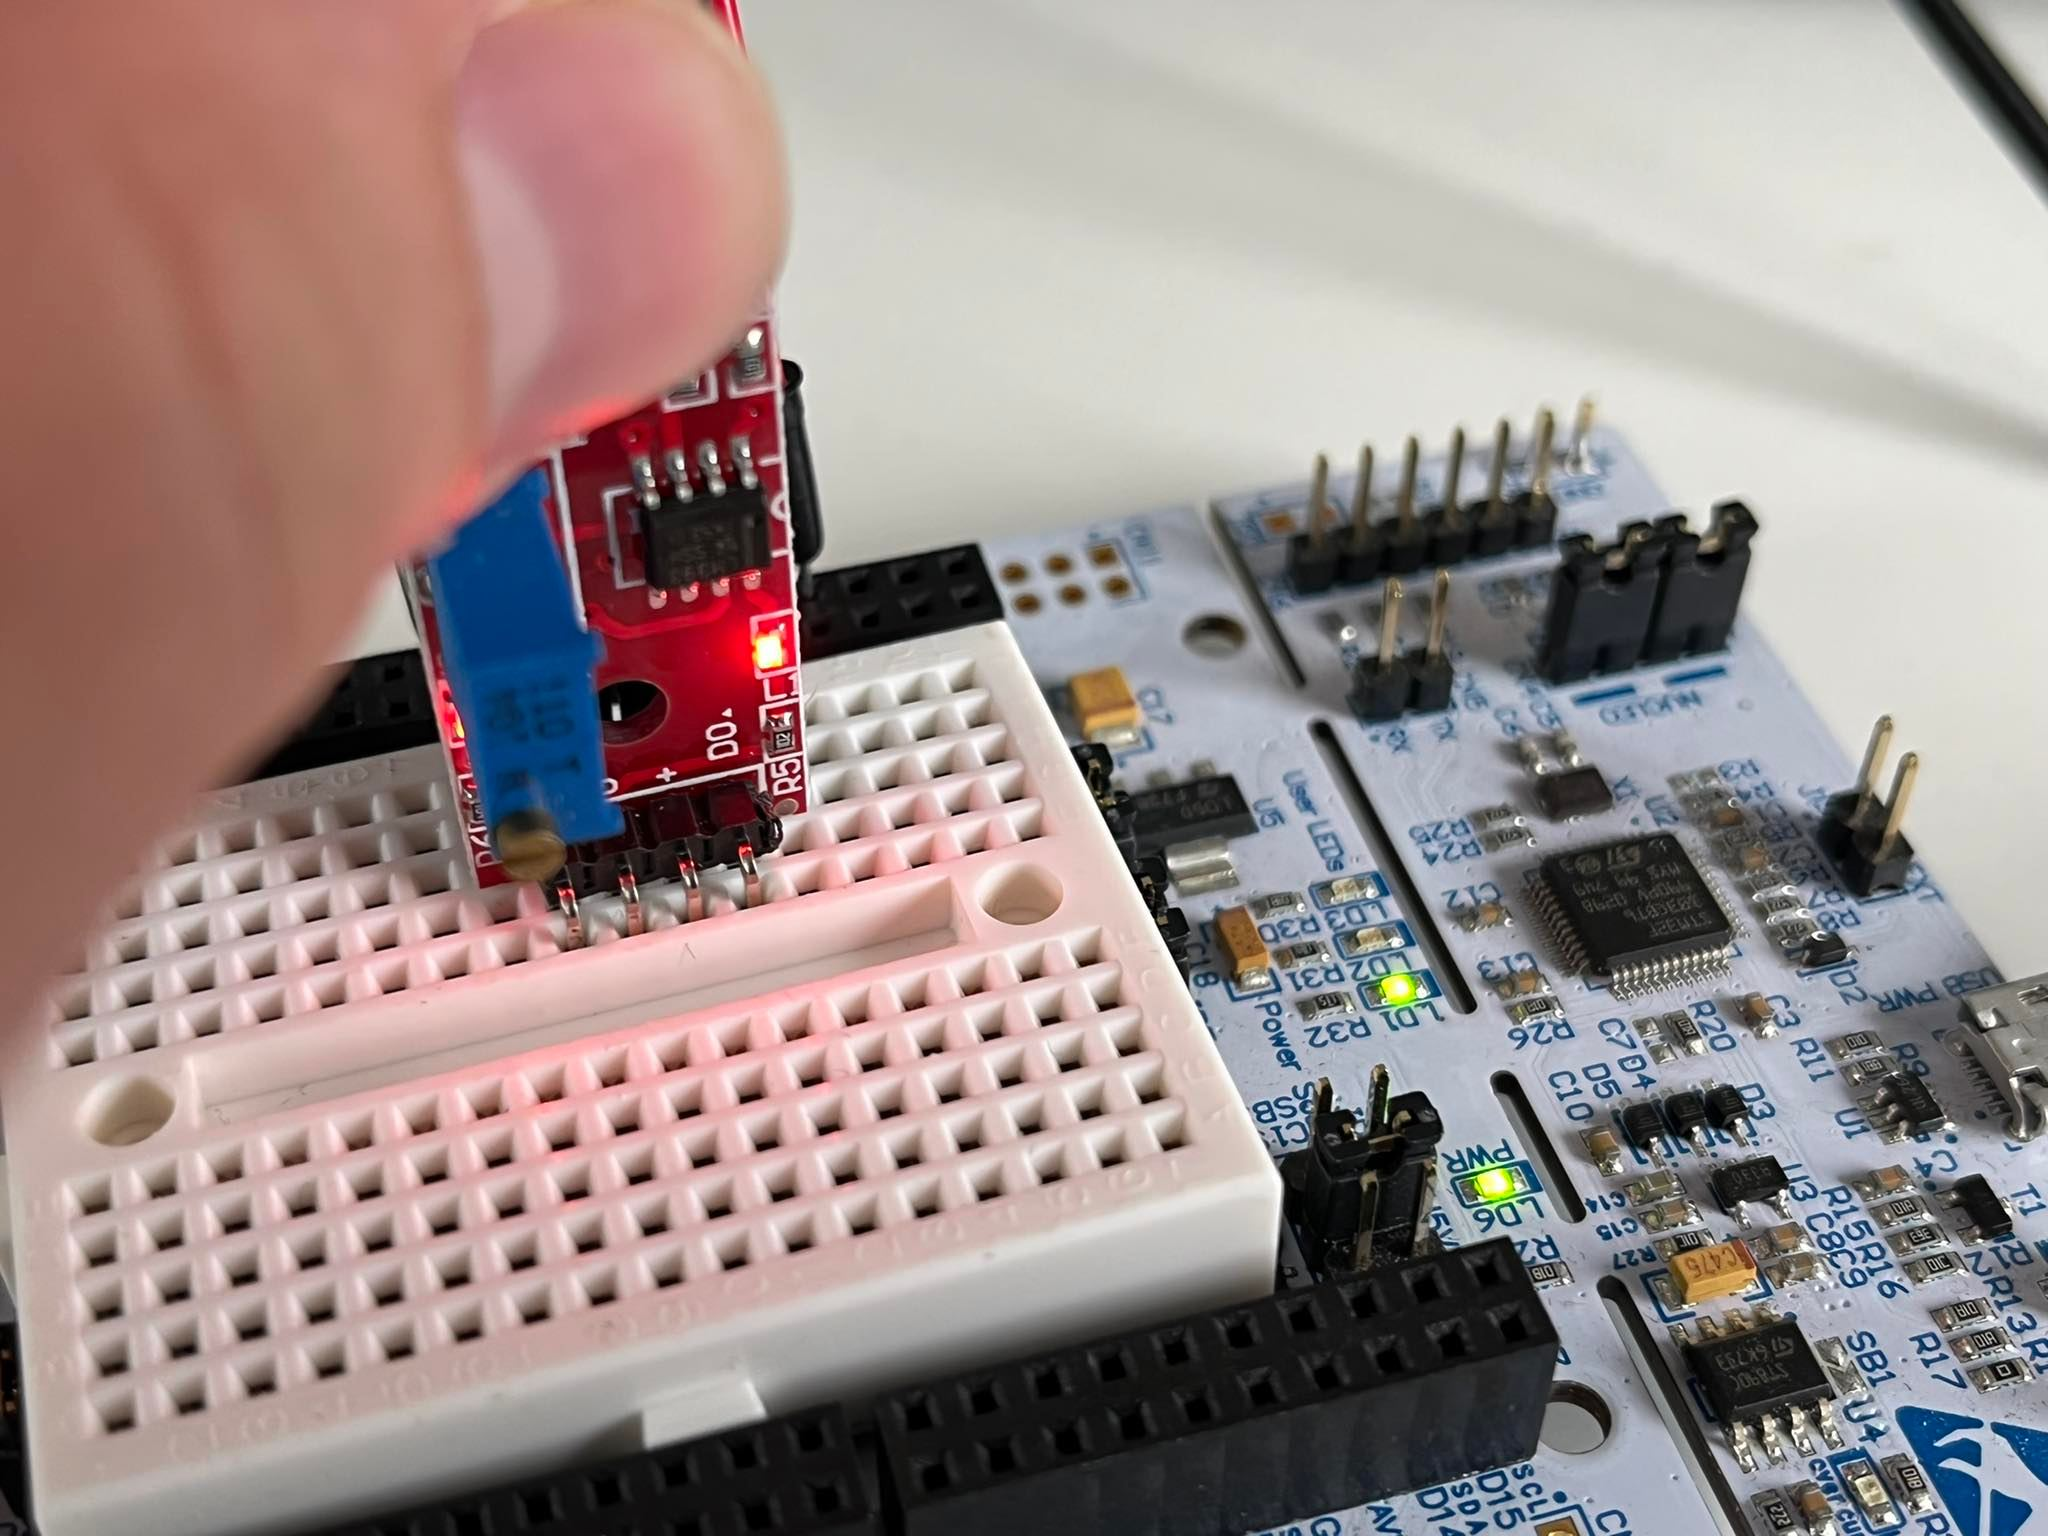
\includegraphics[width=.9\linewidth]{fig/KY-036/281840585_380019084156582_1310010852558564635_n}
\caption{Dioda LD2 włączona podczas dotyku}
\label{fig:_układ_mikroproc_dioda_wla}
\end{subfigure}
%%%%%%%%%%%%%%%%%%%%%%%%%%%%%%%%%%%%%%%%%%%%%%%%%%%%%%%%%%%%%%%%%%%%%%%%%%%%%%%%%
% \caption{PODPIS}
\label{fig:mikroproc}
\end{figure}
\vspace{0.25cm}
%%%%%%%%%%%%%%%%%%%%%%%%%  TWO IMAGES SIDE BY SIDE  %%%%%%%%%%%%%%%%%%%%%%%%%%%%%
\subsection{Wyjście analogowe}
Wbudowany w mikrokontroler przetwornik ADC również pozwala nam obsługować wbudowane wejście analogowe. Należny jednak pamiętać o sprzętowych ograniczeniach pinów. W przypadku mikrokontrolera z rodziny \texttt{STM32 Nucleo} jest to 3.3V, dlatego układ zasilany jest ze źródła napięciowego 3.3V.

\begin{figure}[h!]
    \centering
    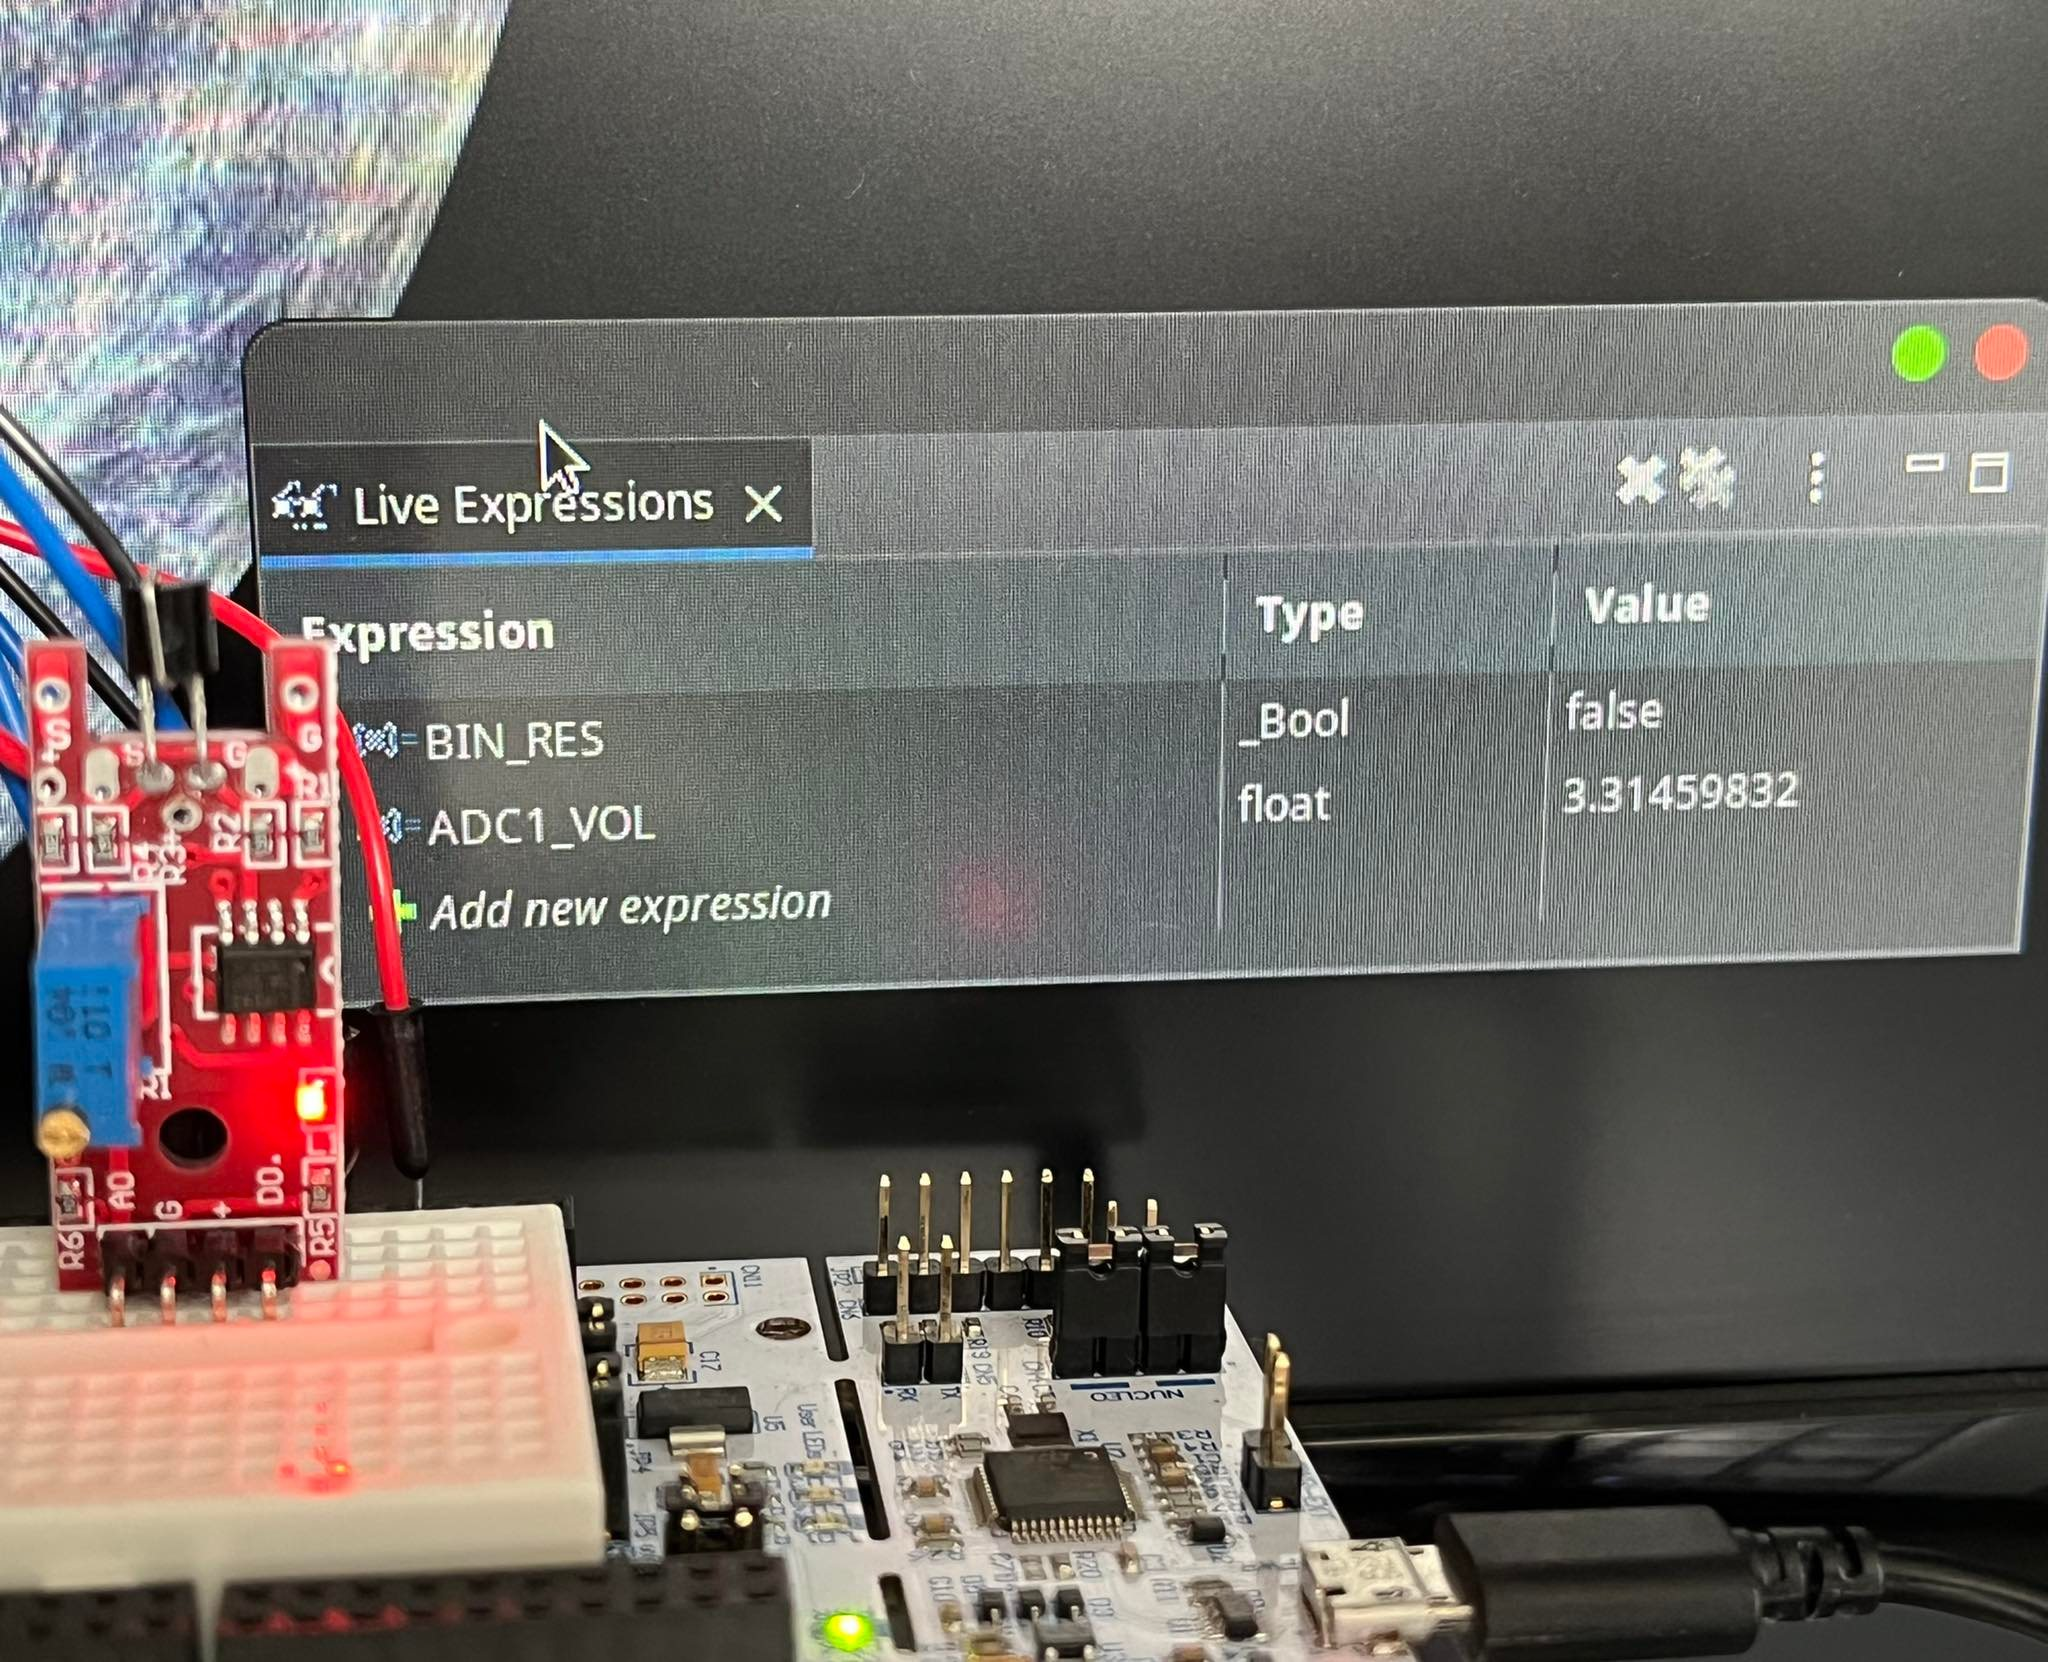
\includegraphics[width=0.6\textwidth]{fig/KY-036/284656287_1051707678886130_4346124543266946166_n}
    \caption{Interfejs analogowy przy użyciu mikokontrolera}
    \label{fig:my_label}
\end{figure}


\newpage
%\printbibliography[heading=bibintoc]

\end{document}